%% template-AutoScaling.tex
%% Author: Zongxu Mu, Yasha Pushak
%% This is the LaTeX template file for Empirical Scaling Analyser (ESA) v1.1.
%% ESA takes the template, replace variables with their corresponding values,
%%	and generates an output file named AutoScaling.tex.
%% You may compile this file alone without running ESA to see how the output looks like.
%% Variables are surrounded by ``@@''s
%% Supported variable names include:
%%	- algName, e.g., ``WalkSAT/SKC''
%%	- instName, e.g., ``random 3SAT at phase transition''
%%	- models, e.g., ``\\begin{itemize}\n\\item $Exp\\left[a,b\\right]\\left(n\\right)=a\\cdot b^{n}$ \\quad{}(2-parameter exponential);\n\\end{itemize}''
%%	- numBootstrapSamples, the number of bootstrap samples used in the analysis, e.g., 1000
%%	- numInsts, the number of instances used in the analysis, e.g., 1200
%%      - numInsts[Train,Test], the number of instances used as support/challenge data in the anlaysis, e.g., 600.
%%	- largestSupportSize, e.g., 500
%%	- table-Details-dataset, e.g., ``\\input{table_Details-dataset}''
%%	- table-Details-dataset, e.g., ``\\input{table_Details-dataset}''
%%	- table-Fitted-models, e.g., ``\\begin{tabular}{ccccc} 
\hline 
 &  & \multirow{2}{*}{Model} & RMSE  & RMSE\tabularnewline 
 &  &  & (support)  & (challenge)\tabularnewline 
\hline 
\hline 
\multirow{3}{*}{p15S363} & EXP. Model & $0.95094\times 1.0017^{x}$ & $0.34618$ & $30.319$ \tabularnewline 
 & Poly. Model & $4.3589\times10^{-8}\times x^{2.675}$ & $0.84016$ & $34.759$ \tabularnewline 
 & SQRTEXP. Model & $\mathbf{0.06958\times 1.145^{\sqrt{x}}}$ & $\mathbf{0.39499}$ & $\mathbf{19.033}$ \tabularnewline 
\hline 
\end{tabular} 

''
%%	- figure-fittedModels, e.g., ``\\includegraphics[width=0.8\textwidth]{fittedModels_loglog}''
%%	- supportSizes, the sizes used for fitting the models, e.g., ``200, 250, 300, 350, 400, 450, 500''
%%	- challengeSizes, e.g., ``600, 700, 800, 900, 1000''
%%	- table-Bootstrap-intervals-of-parameters, e.g., ``\\begin{tabular}{cc|cc} 
\hline 
Solver  & Model  & Confidence interval of $a$  & Confidence interval of $b$ \tabularnewline 
\hline 
\multirow{3}{*}{WalkSAT/SKC} & Exp. & $\left[0.0004476,0.0010113\right]$ & $\left[1.007,1.0091\right]$ \tabularnewline 
 & RootExp. & $\left[1.0905\times10^{-5},6.1897\times10^{-5}\right]$ & $\left[1.3243,1.4433\right]$ \tabularnewline 
 & Poly. & $\left[4.5554\times10^{-12},1.011\times10^{-9}\right]$ & $\left[2.7812,3.6834\right]$ \tabularnewline 
\hline 
\end{tabular} 

''
%%	- table-Bootstrap-intervals, e.g., ``\\input{table_Bootstrap-intervals}''
%%	- analysisSummary, e.g., ``observed median running times are consistent with the polynomial scaling model''
\documentclass[british]{article}
\usepackage[T1]{fontenc}
\usepackage[latin9]{inputenc}
\usepackage{geometry}
\geometry{verbose,tmargin=3.5cm,bmargin=3.5cm,lmargin=3cm,rmargin=3cm}
\usepackage{array}
\usepackage{multirow}
\usepackage{amstext}
\usepackage{graphicx}
\usepackage[usenames, dvipsnames]{color}

\newcommand{\updatedYP}[1]{#1}
\newcommand{\yp}[1]{#1}
\newcommand{\orange}[1]{#1}
\newcommand{\evalModels}[1]{#1}
\newcommand{\bestBoot}[1]{#1}

\newcommand{\medianInterval}[1]{}
\newcommand{\randomizedAlgorithm}[1]{}
@@customCommands@@

\makeatletter

%%%%%%%%%%%%%%%%%%%%%%%%%%%%%% LyX specific LaTeX commands.
%% Because html converters don't know tabularnewline
\providecommand{\tabularnewline}{\\}

%%%%%%%%%%%%%%%%%%%%%%%%%%%%%% User specified LaTeX commands.

\title{On the empirical scaling of running time of @@algName@@ for solving @@instName@@}
\author{Empirical Scaling Analyzer}

\makeatother

\usepackage{babel}
\begin{document}
\maketitle %


\section{Introduction}

This is the automatically generated report on the empirical scaling
of the running time of @@algName@@ for solving @@instName@@.


\section{Methodology} %TODO: Update entire section

\label{sec:Methodology}

% models, model fitting
For our scaling analysis, we considered the following parametric models:
@@models@@
% \begin{itemize}
% \item $Exp\left[a,b\right]\left(n\right)=a\cdot b^{n}$ \quad{}(2-parameter exponential); 
% \item $RootExp\left[a,b\right]\left(n\right)=a\cdot b^{\sqrt{n}}$ \quad{}(2-parameter root-exponential); 
% \item $Poly\left[a,b\right]\left(n\right)=a\cdot n^{b}$ \quad{}(2-parameter polynomial). 
% \end{itemize}
Note that the approach could be easily extended to other scaling models.
For fitting parametric scaling models to observed data, we used the
non-linear least-squares Levenberg-Marquardt algorithm. 

% what we fitted the models to, how we assessed model fit
Models were fitted to performance observations in the form of @@statistic@@s
of the distributions of running times over sets of instances for given
$n$, the instance size.
\randomizedAlgorithm{
Since @@algName@@ is a randomized algorithm, we analyzed the per-instance @@perInstanceStatistic@@ of @@numRunsPerInstance@@ independent runs for each instance. This means that models were fitted to @@statistic@@s of per-instance @@perInstanceStatistic@@s. Similarly, the running time statistics reported throughout this report are statistics of per-instance @@perInstanceStatistic@@s. 
}
%Compared to the mean, the median has two
%advantages: it is statistically more stable and immune to the presence
%of a certain amount of timed-out runs.
To assess the fit of a given
scaling model to observed data, we used root-mean-square error (RMSE). 

\medianInterval{
Due to the instances for which the running times are unknown, 
there is uncertainty about the
precise location of the @@statistic@@s of the running time distributions
at each such $n$, and we can only provide bounds on
those @@statistic@@s instead. Closely following \cite{dubois2015on}, we calculate
these bounds based on the best-and worst-case scenarios, in which all instances with unknown running times
are easiest or hardest, respectively.
We note that these are not confidence
intervals, since we can guarantee the actual @@statistic@@ running
times to lie within them.
We also calculate RMSEs and confidence intervals based on these bounds.
}

% bootstrap confidence intervals
Closely following \cite{hoos2009bootstrap,hoos2014empirical}, we
computed 95\% bootstrap confidence intervals for the performance predictions
obtained from our scaling models, based on @@numBootstrapSamples@@ bootstrap samples
per instance set and @@numBootstrapSamples@@ automatically fitted variants of each scaling
model. 
\bestBoot{To extend this idea, we calculated support and challenge RMSEs for each of the fitted models' predictions and the corresponding
bootstrap samples of the observed data. We used these bootstrap sample
RMSEs to calculate median and 95\% confidence intervals of the support and challenge RMSEs for each model. 
\medianInterval{In order to handle the unknown running times, we used the geometric means of the @@statistic@@ intervals for each instance size to calculate the median RMSEs.
However, to better capture both sources of uncertainty for the bootstrap intervals, we calculated the RMSE interval upper and lower bounds by computing 97.5 and 2.5 quantiles
for the set of upper bounds and the set of lower bounds on the RMSEs, respectively.}}
\randomizedAlgorithm{Since this analysis was performed on per-instance @@perInstanceStatistic@@s, we also computed these statistics on nested, per-instance bootstrap samples, by first computing @@perInstanceStatistic@@s for @@numPerInstanceBootstrapSamples@@ bootstrap samples for each instance and then randomly selecting one of the per-instance @@perInstanceStatistic@@s when needed.}


\updatedYP{
In the following, we say that a scaling model prediction is in-consistent 
with observed data if the bootstrap confidence interval for the observed data
is disjoint from the bootstrap confidence interval for the
predicted @@statistic@@ \randomizedAlgorithm{of per-instance 
@@perInstanceStatistic@@}
 running times; we say that a scaling model prediction is weakly consistent 
with the observed data if the bootstrap confidence interval for the prediction overlaps with the bootstrap confidence interval for the observed data;
%\medianInterval{we say that a scaling model prediction is consistent 
%with observed data, if the interval for observed @@statistic@@ \randomizedAlgorithm{of per-instance @@perInstanceStatistic@@} running times
%overlaps with the
%bootstrap confidence interval for predicted running times;} 
and, we say that a scaling model is strongly consistent with observed
data, if the bootstrap confidence interval for the observed @@statistic@@ \randomizedAlgorithm{of per-instance @@perInstanceStatistic@@s} is fully contained
within the bootstrap confidence interval for predicted
running times.}
Also, we define the residue of a model at a given size as the observed 
point estimate less the predicted value.


\section{Dataset Description}

The dataset contains running times of the @@algName@@ algorithm solving
@@numInsts@@ instances of different sizes \randomizedAlgorithm{with @@numRunsPerInstance@@ independent runs per instance}. We split the running times into
two categories, support ($n\leq@@largestSupportSize@@$) and challenge ($n>@@largestSupportSize@@$) with @@numInstsTrain@@ and @@numInstsTest@@, respectively.. The
details of the dataset can be found in Tables \ref{tab:Details-dataset-support} 
and \ref{tab:Details-dataset-challenge}.
\begin{table*}
\noindent \begin{centering}
@@table-Details-dataset-support@@
\par\end{centering}

\caption{\label{tab:Details-dataset-support} Details of the running time dataset used as support data for model fitting. \randomizedAlgorithm{The reported statistics are of the per-instance @@perInstanceStatistic@@ running times.}}
\end{table*}

\begin{table*}
\noindent \begin{centering}
@@table-Details-dataset-challenge@@
\par\end{centering}

\caption{\label{tab:Details-dataset-challenge} Details of the running time dataset used as challenge data for model fitting. \randomizedAlgorithm{The reported statistics are of the per-instance @@perInstanceStatistic@@ running times.}}
\end{table*}

% 
% Figure \ref{fig:CDFs} shows the distributions of the running times of
% @@algName@@ solving @@instName@@. 
% \begin{figure*}[tb]
% \begin{centering}
% @@figure-cdfs@@
% % \includegraphics[width=0.8\textwidth]{cdfs}  
% \par\end{centering}
% 
% \noindent \centering{}\caption{\label{fig:CDFs} Distribution of running times across instance sets for
% @@algName@@.}
% \end{figure*}
% 
% 

\section{Empirical Scaling of Solver Performance}

\label{sec:Results}

We first fitted our parametric scaling models to the @@statistic@@s of the \randomizedAlgorithm{per-instance @@perInstanceStatistic@@} running times
of @@algName@@, as described in Section \ref{sec:Methodology}. The
models were fitted using the @@statistic@@s of the \randomizedAlgorithm{per-instance @@perInstanceStatistic@@} running times for $@@supportSizes@@$
(support) and later challenged with the @@statistic@@s of the \randomizedAlgorithm{per-instance @@perInstanceStatistic@@} running times for $@@challengeSizes@@$.
This resulted in the models, shown along with RMSEs on support and
challenge data, shown in Table~\ref{tab:Fitted-models}.
\begin{table}[tb]
\begin{centering}
@@table-Fitted-models@@
% \begin{tabular}{ccccc} 
\hline 
 &  & \multirow{2}{*}{Model} & RMSE  & RMSE\tabularnewline 
 &  &  & (support)  & (challenge)\tabularnewline 
\hline 
\hline 
\multirow{3}{*}{p15S363} & EXP. Model & $0.95094\times 1.0017^{x}$ & $0.34618$ & $30.319$ \tabularnewline 
 & Poly. Model & $4.3589\times10^{-8}\times x^{2.675}$ & $0.84016$ & $34.759$ \tabularnewline 
 & SQRTEXP. Model & $\mathbf{0.06958\times 1.145^{\sqrt{x}}}$ & $\mathbf{0.39499}$ & $\mathbf{19.033}$ \tabularnewline 
\hline 
\end{tabular} 


\par\end{centering}

\caption{\label{tab:Fitted-models}Fitted models of the @@statistic@@s of the \randomizedAlgorithm{per-instance @@perInstanceStatistic@@} running times and RMSE
values (in CPU sec). The models yielding the most
accurate predictions (as per RMSEs on challenge data) are shown in
boldface.}
\end{table}
In addition, we illustrate the fitted models of @@algName@@ in Figure~\ref{fig:Fitted-models},
and the residues for the models in Figure~\ref{fig:Fitted-residues}.
\begin{figure}[tb]
\noindent \begin{centering}
@@figure-fittedModels@@
% 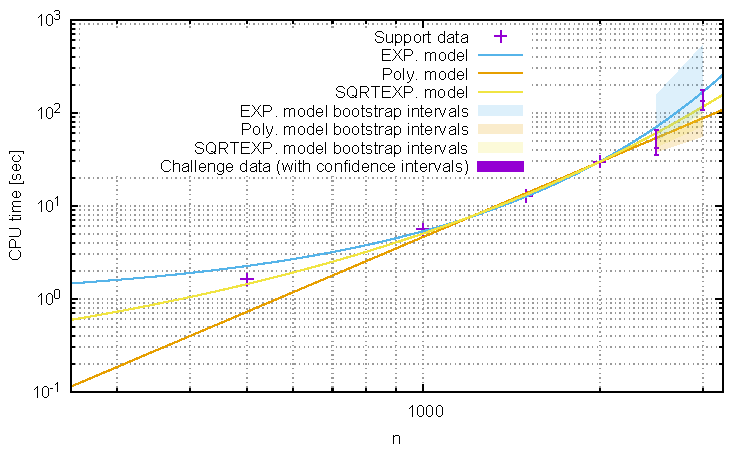
\includegraphics[width=0.8\textwidth]{fittedModels}
\par\end{centering}

\caption{\label{fig:Fitted-models} Fitted models of the @@statistic@@s of the \randomizedAlgorithm{per-instance @@perInstanceStatistic@@} running times. 
The models are fitted with the @@statistic@@s of the \randomizedAlgorithm{per-instance @@perInstanceStatistic@@} running times of
@@algName@@ solving the set of @@instName@@ 
of $@@supportSizes@@$ variables, and are challenged by the @@statistic@@s of the \randomizedAlgorithm{per-instance @@perInstanceStatistic@@}
running times of $@@challengeSizes@@$ variables.}
\end{figure}


\begin{figure}[tb]
\noindent \begin{centering}
@@figure-fittedResidues@@
% 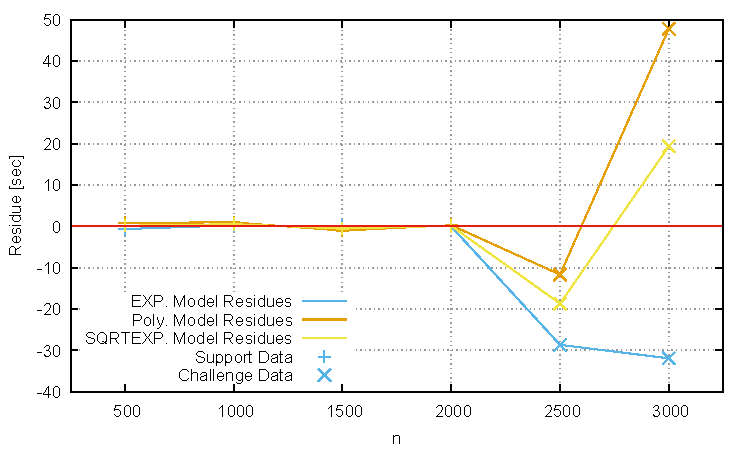
\includegraphics[width=0.8\textwidth]{fittedResidues}
\par\end{centering}

\caption{\label{fig:Fitted-residues} Residues of the fitted models of the @@statistic@@s of the \randomizedAlgorithm{per-instance @@perInstanceStatistic@@} running times. }
\end{figure}


But how much confidence should we have in these models? Are the RMSEs
small enough that we should accept them? To answer this question,
we assessed the fitted models using the bootstrap approach outlined
in Section~\ref{sec:Methodology}. Table~\ref{tab:Bootstrap-intervals-of-parameters}
shows the bootstrap intervals of the model parameters, 
\bestBoot{Table~\ref{tab:Bootstrap-model-RMSE} 
shows the bootstrap intervals of the model prediction RMSEs},
and Table~\ref{tab:Bootstrap-intervals-support}
contains the bootstrap intervals for the support data.
Challenging the models with extrapolation, as shown in 
\evalModels{Table~\ref{tab:Bootstrap-intervals-challenge}, it is concluded that
@@analysisSummary@@
(as also illustrated in Figure~\ref{fig:Fitted-models}).
@@analysisSummaryExplaination@@}
\begin{table*}[tb]
\noindent \begin{centering}
@@table-Bootstrap-intervals-of-parameters@@
% \begin{tabular}{cc|cc} 
\hline 
Solver  & Model  & Confidence interval of $a$  & Confidence interval of $b$ \tabularnewline 
\hline 
\multirow{3}{*}{WalkSAT/SKC} & Exp. & $\left[0.0004476,0.0010113\right]$ & $\left[1.007,1.0091\right]$ \tabularnewline 
 & RootExp. & $\left[1.0905\times10^{-5},6.1897\times10^{-5}\right]$ & $\left[1.3243,1.4433\right]$ \tabularnewline 
 & Poly. & $\left[4.5554\times10^{-12},1.011\times10^{-9}\right]$ & $\left[2.7812,3.6834\right]$ \tabularnewline 
\hline 
\end{tabular} 



\par\end{centering}
\caption{\label{tab:Bootstrap-intervals-of-parameters} 95\% bootstrap intervals
of model parameters for the @@statistic@@s of the \randomizedAlgorithm{per-instance @@perInstanceStatistic@@} running times}

%Group tables 4 and 5 together. 
%\end{table*}
%\begin{table*}[tb]
\bigskip

\noindent \begin{centering}
@@table-Bootstrap-model-Loss@@
% \input{table_Bootstrap-model-Loss}

\par\end{centering}
\caption{\label{tab:Bootstrap-model-RMSE} \bestBoot{95\% bootstrap confidence intervals
of model prediction losses for the @@statistic@@s of the \randomizedAlgorithm{per-instance @@perInstanceStatistic@@} running times.%
%\medianInterval{To calculate the median RMSEs we used the geometric mean of the intervals for the @@statistic@@s of 
%the \randomizedAlgorithm{per-instance @@perInstanceStatistic@@} running times for each instance size. However, the bootstrap 
%confidence intervals directly capture both sources of uncertainty by reporting the 2.5 and 97.5 
%quantiles of the lower and upper bounds on the RMSEs, respectively.} 
@@winnerSelectRule@@ }}
\end{table*}


\begin{table*}[tb]
\noindent \begin{centering}
@@table-Bootstrap-intervals-support@@
% \input{table_Bootstrap-intervals}
\par\end{centering}

\caption{\label{tab:Bootstrap-intervals-support} 95\% bootstrap confidence intervals
for the @@statistic@@s of the \randomizedAlgorithm{per-instance @@perInstanceStatistic@@} running time predictions and observed running times on @@instName@@. 
The instance sizes shown here are those used for fitting the models.
Bootstrap intervals on predictions that are weakly consistent
with the observed point estimates are shown in boldface 
%\medianInterval{those that are consistent are marked by plus signs ({+}),}
and those that are strongly consistent are marked
by asterisks ({*}).}
%and those that fully contain the confidence intervals on 
%observations are marked by asterisks ({*}).}
\end{table*}

\begin{table*}[tb]
\noindent \begin{centering}
@@table-Bootstrap-intervals-challenge@@
% \input{table_Bootstrap-intervals}
\par\end{centering}

\caption{\label{tab:Bootstrap-intervals-challenge} 95\% bootstrap confidence intervals
for the @@statistic@@s of the \randomizedAlgorithm{per-instance @@perInstanceStatistic@@} running time predictions and observed running times on @@instName@@. 
The instance sizes shown here are larger than those used for fitting the models.
Bootstrap intervals on predictions that are weakly consistent
with the observed data are shown in boldface
%\medianInterval{those that are consistent are marked by plus signs ({+}),}
and those that are strongly consistent are marked
by asterisks ({*}).}
%and those that fully contain the confidence intervals on 
%observations are marked by asterisks ({*}).}
\end{table*}


\section{Conclusion}

In this report, we presented an empirical analysis of the scaling
behaviour of @@algName@@ on @@instName@@. We found
@@analysisSummary@@.

\bibliographystyle{plain}
\begin{thebibliography}{1}

\bibitem{dubois2015on}
J{\'e}r{\'e}mie Dubois-Lacoste, Holger~H. Hoos, and Thomas St{\"u}tzle.
\newblock On the empirical scaling behaviour of state-of-the-art local search
  algorithms for the {E}uclidean {TSP}.
\newblock In {\em Proceedings of the 17th Genetic and Evolutionary Computation Conference}, (GECCO '15), pages 377--384, 2015.

\bibitem{hoos2009bootstrap}
Holger~H. Hoos.
\newblock A bootstrap approach to analysing the scaling of empirical run-time
  data with problem size.
\newblock Technical report, Technical Report TR-2009-16, Department of Computer Science, University of British
  Columbia, 2009.

\bibitem{hoos2014empirical}
Holger~H. Hoos and Thomas St{\"u}tzle.
\newblock On the empirical scaling of run-time for finding optimal solutions to
  the travelling salesman problem.
\newblock {\em European Journal of Operational Research}, 238(1):87--94, 2014.

\end{thebibliography}

\end{document}
